%\documentclass[]{beamer}
\documentclass[handout]{beamer}
%\usepackage[dvips]{color}
\usepackage{graphicx}
\usepackage{amsmath,amssymb,array,comment,eucal}
\usepackage{xcolor}
\definecolor{beamer@blendedblue}{RGB}{86,155,189}
\definecolor{myblue}{RGB}{12,76,138}
\setbeamercolor{structure}{fg=myblue}
\definecolor{Ftitle}{RGB}{12,76,138}
\definecolor{Descitem}{RGB}{238,238,244}
\definecolor{StdTitle}{RGB}{12,76,138}
\definecolor{StdBody}{RGB}{213,24,0}
\definecolor{StdBody}{RGB}{213,24,0}

\definecolor{AlTitle}{RGB}{255, 190, 190}
\definecolor{AlBody}{RGB}{213,24,0}

\definecolor{ExTitle}{RGB}{201, 217, 217}
\definecolor{ExBody}{RGB}{213,24,0}

\setbeamercolor{frametitle}{fg = Ftitle}
\setbeamercolor{title}{fg = Ftitle}
\setbeamercolor{item}{fg = Ftitle}
\setbeamercolor{subitem}{fg = Ftitle}
\setbeamercolor{subsubitem}{fg = Ftitle}
\setbeamercolor{description item}{fg = myblue}
\setbeamercolor{titlelike}{fg=myblue}

\DeclareMathOperator{\sgn}{sgn}
\newcommand{\e}{\mathbf{e}}
\renewcommand{\P}{\mathbf{P}}
\newcommand{\F}{\mathbf{F}}
\newcommand{\R}{\textsf{R}}
\newcommand{\mat}[1] {\mathbf{#1}}
%\newcommand{\ind}{\mathrel{\mathop{\sim}\limits^{\mathit{ind}}}}
%\newcommand{\iid}{\mathrel{\mathop{\sim}\limits^{\mathit{iid}}}}
\newcommand{\E}{\textsf{E}}
\newcommand{\SE}{\textsf{SE}}
\newcommand{\SSE}{\textsf{SSE}}
\newcommand{\RSS}{\textsf{RSS}}
\newcommand{\FSS}{\textsf{FSS}}
\renewcommand{\SS}{\textsf{SS}}
\newcommand{\MSE}{\textsf{MSE}}
\newcommand{\SSR}{\textsf{SSR}}
\newcommand{\Be}{\textsf{Beta}}
\newcommand{\St}{\textsf{St}}
\newcommand{\Ca}{\textsf{C}}
\newcommand{\Exp}{\textsf{Exp}}
\newcommand{\GDP}{\textsf{GDP}}
\newcommand{\NcSt}{\textsf{NcSt}}
\newcommand{\Bin}{\textsf{Bin}}
\newcommand{\NB}{\textsf{NegBin}}
\renewcommand{\NG}{\textsf{NG}}
\newcommand{\N}{\textsf{N}}
\newcommand{\Ber}{\textsf{Ber}}
\newcommand{\Poi}{\text{Poi}}
\newcommand{\Gam}{\textsf{Gamma}}
\newcommand{\BB}{\textsf{BB}}
\newcommand{\Gm}{\textsf{G}}
\newcommand{\Un}{\textsf{Unif}}
\newcommand{\Ex}{\textsf{Exp}}
\newcommand{\DE}{\textsf{DE}}
\newcommand{\tr}{\textsf{tr}}
\newcommand{\cF}{{\cal{F}}}
\newcommand{\cL}{{\cal{L}}}
\newcommand{\cI}{{\cal{I}}}
\newcommand{\cB}{{\cal{B}}}
\newcommand{\cP}{{\cal{P}}}
\newcommand{\bbR}{\mathbb{R}}
\newcommand{\bbN}{\mathbb{N}}
\newcommand{\pperp}{\mathrel{{\rlap{$\,\perp$}\perp\,\,}}}
\newcommand{\OFP}{(\Omega,\cF, \P)}
\newcommand{\eps}{\boldsymbol{\epsilon}}
\newcommand{\1}{\mathbf{1}_n}
\newcommand{\gap}{\vspace{8mm}}
\newcommand{\ind}{\mathrel{\mathop{\sim}\limits^{\rm ind}}}
\newcommand{\simiid}{\ensuremath{\mathrel{\mathop{\sim}\limits^{\rm
iid}}}}
\newcommand{\eqindis}{\ensuremath{\mathrel{\mathop{=}\limits^{\rm D}}}}
\newcommand{\iid}{\textit{i.i.d.}}
\newcommand{\SSZ}{S_{zz}}
\newcommand{\SZW}{S_{zw}}
\newcommand{\Var}{\textsf{Var}}
\newcommand{\corr}{\textsf{corr}}
\newcommand{\diag}{\textsf{diag}}
\newcommand{\var}{\textsf{var}}
\newcommand{\Cov}{\textsf{Cov}}
\newcommand{\Sam}{{\cal S}}
\def\H{\mathbf{H}}
\newcommand{\I}{\mathbf{I}}
\newcommand{\Y}{\mathbf{Y}}
\newcommand{\tY}{\tilde{\mathbf{Y}}}
\newcommand{\Yhat}{\hat{\mathbf{Y}}}
\newcommand{\Yobs}{\mathbf{Y}_{{\cal S}}}
\newcommand{\barYobs}{\bar{Y}_{{\cal S}}}
\newcommand{\barYmiss}{\bar{Y}_{{\cal S}^c}}
\def\bv{\mathbf{b}}
\def\X{\mathbf{X}}
\def\tX{\tilde{\mathbf{X}}}
\def\x{\mathbf{x}}
\def\xbar{\bar{\mathbf{x}}}
\def\Xbar{\bar{\mathbf{X}}}
\def\Xg{\mathbf{X}_{\boldsymbol{\gamma}}}
\def\Ybar{\bar{\Y}}
\def\ybar{\bar{y}}
\def\y{\mathbf{y}}
\def\Yf{\mathbf{Y_f}}
\def\W{\mathbf{W}}
\def\L{\mathbf{L}}
\def\w{\mathbf{w}}
\def\U{\mathbf{U}}
\def\V{\mathbf{V}}
\def\Q{\mathbf{Q}}
\def\Z{\mathbf{Z}}
\def\z{\mathbf{z}}
\def\v{\mathbf{v}}
\def\u{\mathbf{u}}

\def\zero{\mathbf{0}}
\newcommand{\one}{\mathbf{1}}
\newcommand{\taub}{\boldsymbol{\tau}}
\newcommand{\betav}{\boldsymbol{\beta}}
\newcommand{\alphav}{\boldsymbol{\alpha}}
\newcommand{\A}{\mathbf{A}}
\def\a{\mathbf{a}}
\def\K{\mathbf{K}}
\newcommand{\B}{\mathbf{B}}
\def\b{\boldsymbol{\beta}}
\def\bhat{\hat{\boldsymbol{\beta}}}
\def\btilde{\tilde{\boldsymbol{\beta}}}
\def\tb{\boldsymbol{\theta}}
\def\bg{\boldsymbol{\beta_\gamma}}
\def\bgnot{\boldsymbol{\beta_{(-\gamma)}}}
\def\mub{\boldsymbol{\mu}}
\def\tmub{\tilde{\boldsymbol{\mu}}}
\def\muhat{\hat{\boldsymbol{\mu}}}
\def\tb{\boldsymbol{\theta}}
\def\tk{\boldsymbol{\theta}_k}
\def\tj{\boldsymbol{\theta}_j}
\def\Mk{\boldsymbol{{\cal M}}_k}
\def\M{\boldsymbol{{\cal M}}}
\def\Mj{\boldsymbol{{\cal M}}_j}
\def\Mi{\boldsymbol{{\cal M}}_i}
\def\Mg{{\boldsymbol{{\cal M}_\gamma}}}
\def\Mnull{\boldsymbol{{\cal M}}_{N}}
\def\gMPM{\boldsymbol{\gamma}_{\text{MPM}}}
\def\gHPM{\boldsymbol{\gamma}_{\text{HPM}}}
\def\Mfull{\boldsymbol{{\cal M}}_{F}}
\def\tg{\boldsymbol{\theta}_{\boldsymbol{\gamma}}}
\def\g{\boldsymbol{\gamma}}
\def\eg{\boldsymbol{\eta}_{\boldsymbol{\gamma}}}
\def\G{\mathbf{G}}
\def\cM{\cal M}
\def\D{\Delta}
\def \shat{{\hat{\sigma}}^2}
\def\uv{\mathbf{u}}
\def\l {\lambda}
\def\d{\delta}
\def\Sigmab{\boldsymbol{\Sigma}}
\def\Lambdab{\boldsymbol{\Lambda}}
\def\lambdab{\boldsymbol{\lambda}}
\def\Mg{{\cal M}_\gamma}
\def\S{{\cal{S}}}
\def\qg{p_{\boldsymbol{\gamma}}}
\def\pg{p_{\boldsymbol{\gamma}}}
%\def\t{\mathbf{t}}
\def\T{\boldsymbol{\Theta}}
\def\Tb{\boldsymbol{\Theta}}

\usepackage{verbatim}


\title{Outliers \& Robust Bayesian  Regression}

\author{STA 702 Duke University}

\subtitle{Readings: Hoff Chapter 9, West JRSSB 1984, F{\'{u}}quene,
    P{\'e}rez \& Pericchi 2015}


\institute{Duke University}
\date{\today}
\logo{duke.eps}

\usepackage{Sweave}
\begin{document}
\Sconcordance{concordance:18-outliers.tex:18-outliers.Rnw:%
1 21 1 1 0 328 1}

\maketitle

% -------
\begin{frame}{Body Fat Data: Intervals w/ All Data}
Response \% Body Fat and Predictor Waist Circumference

  \begin{tabular}{cc}
{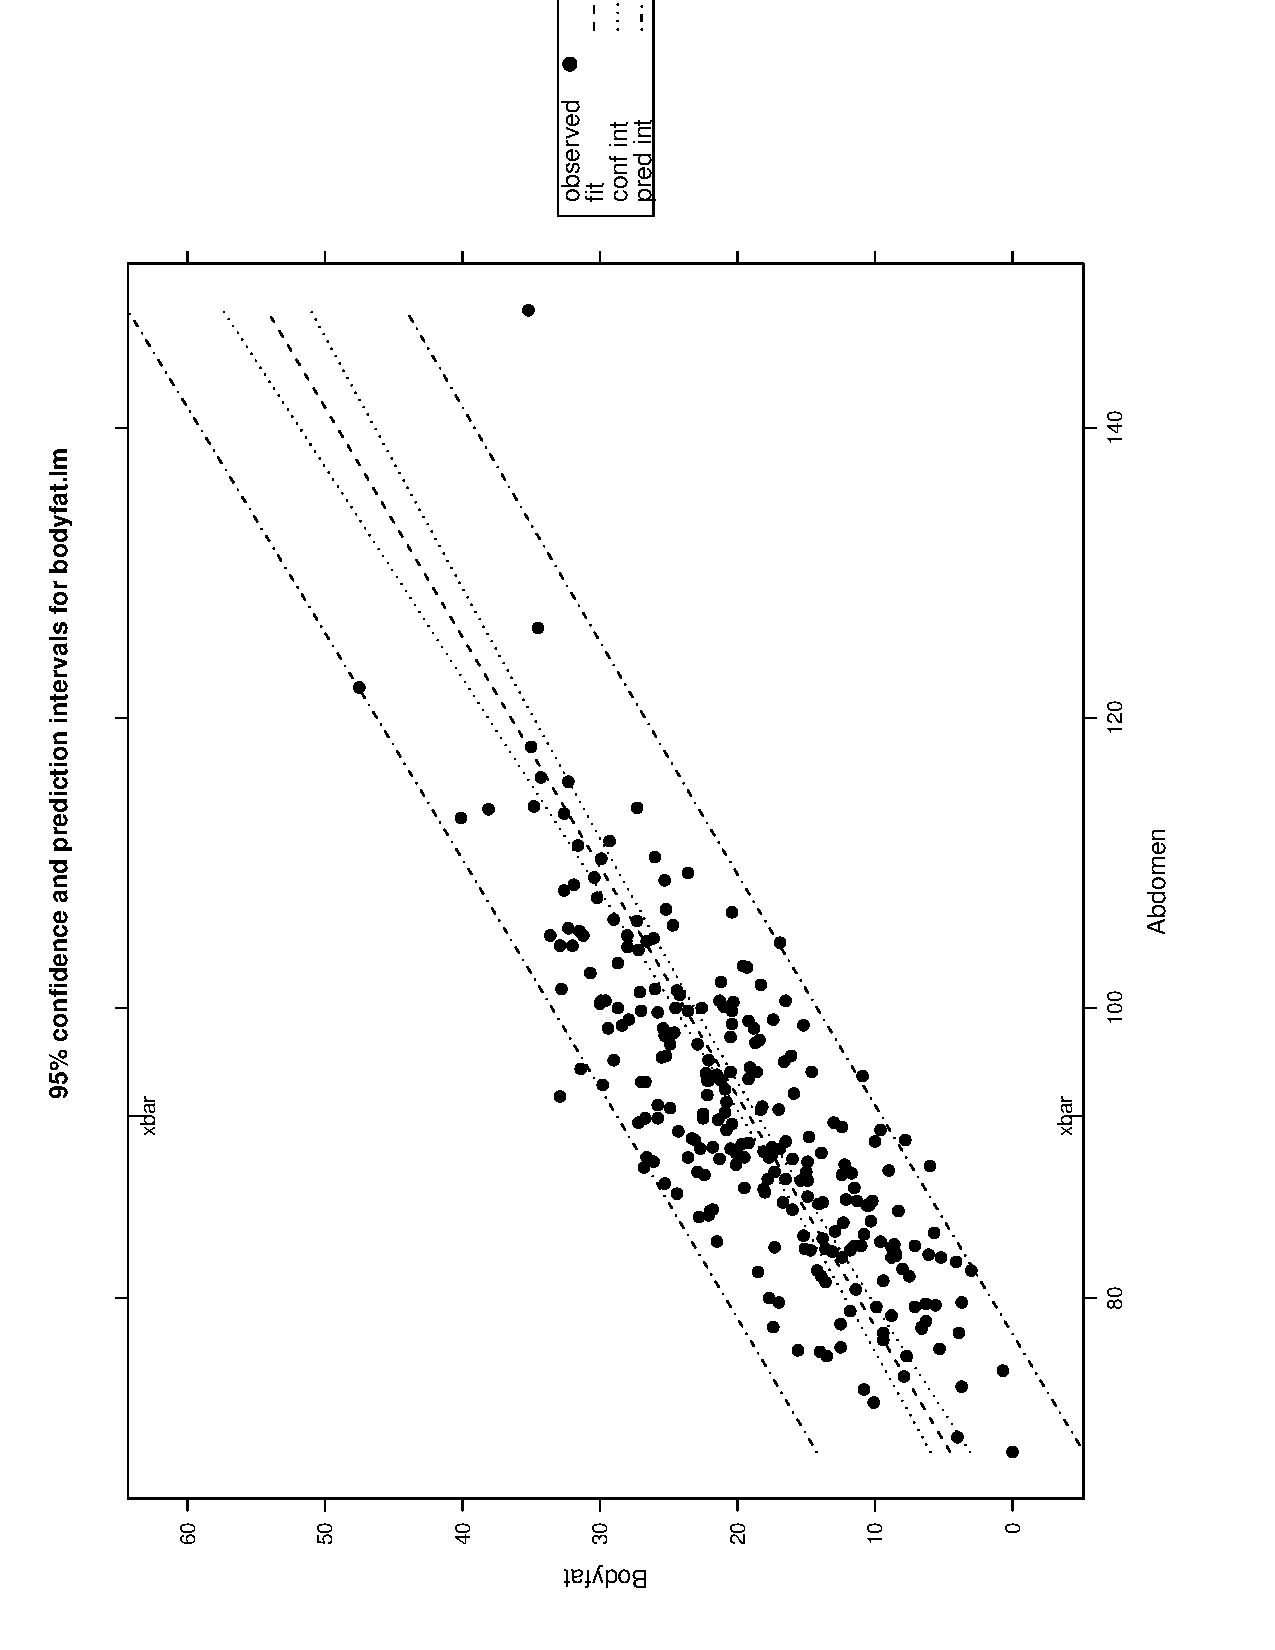
\includegraphics[height=2.in,angle=270]{pred}} &
{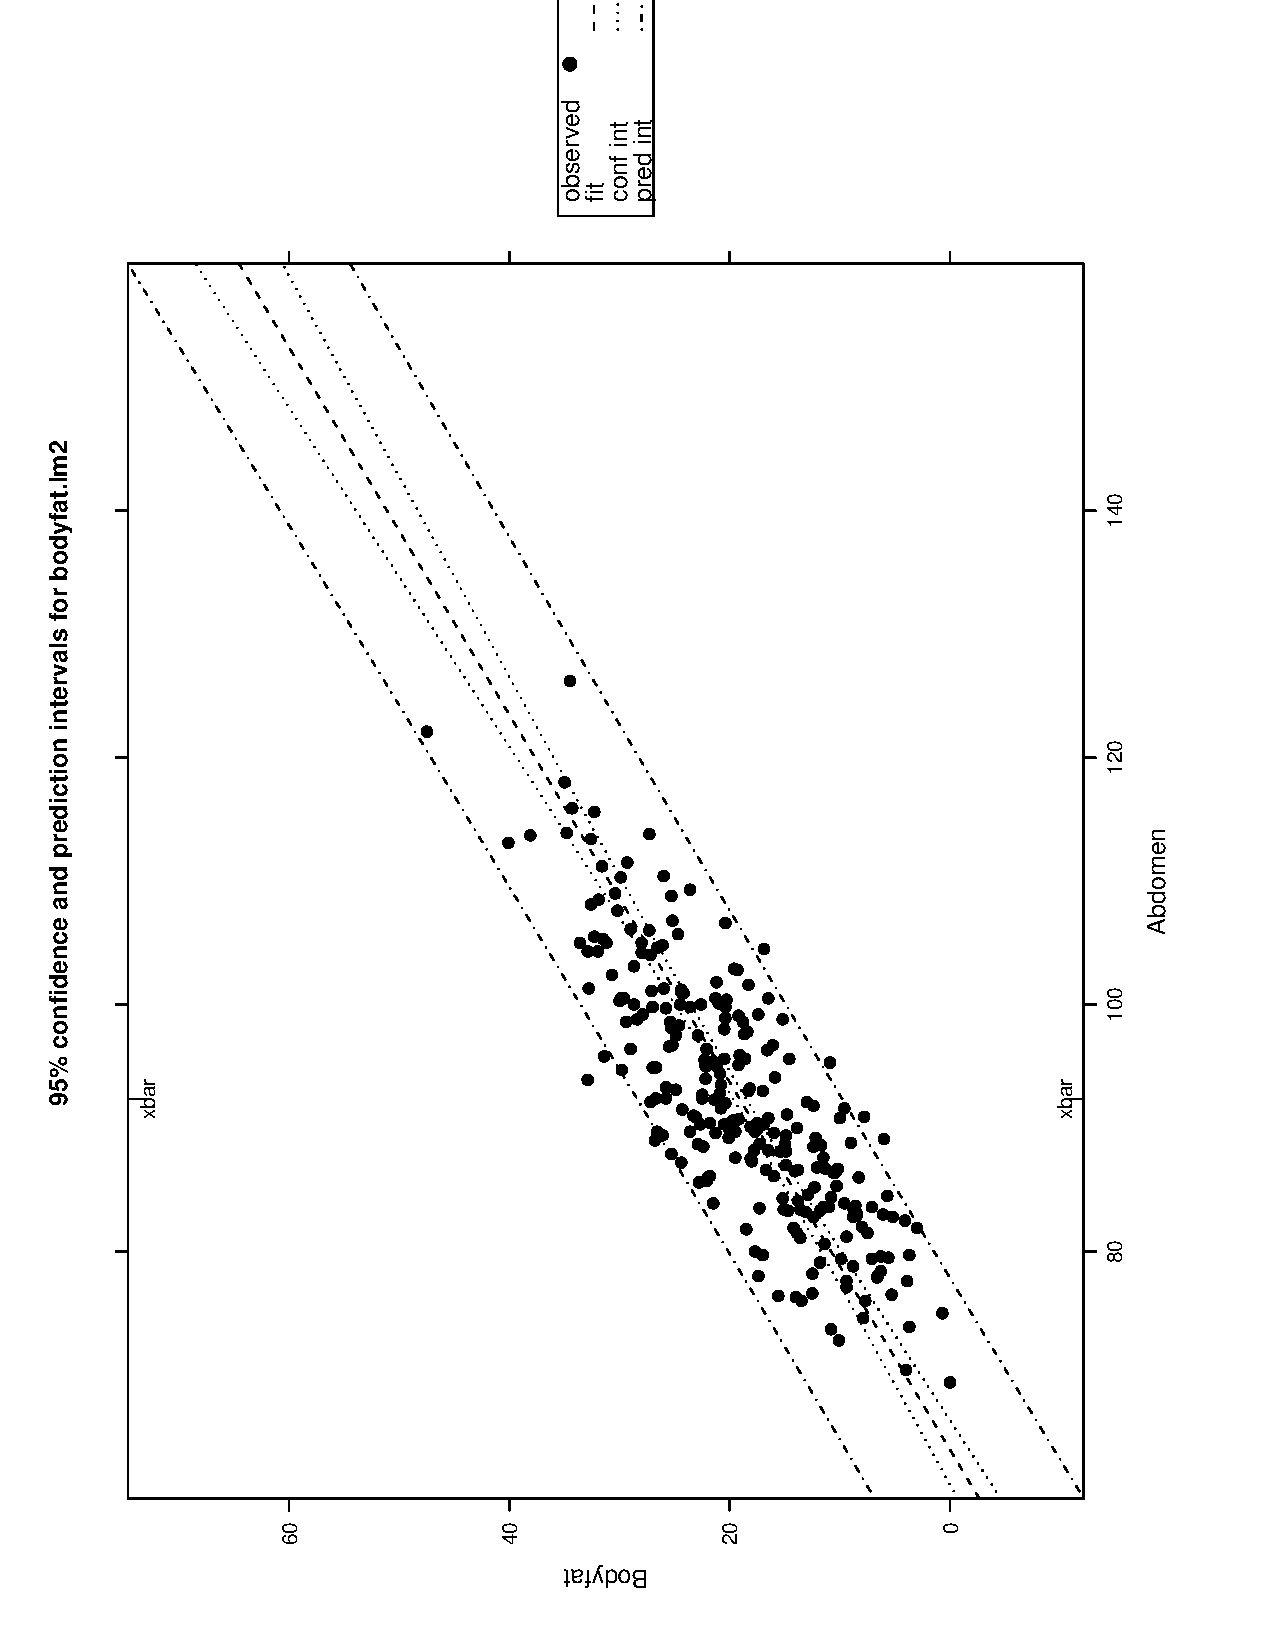
\includegraphics[height=2.in,angle=270]{pred-sub}}
  \end{tabular}

  Which analysis do we use?  with Case 39 or not -- or something different?


\end{frame}  \begin{frame} \frametitle{Cook's Distance}

{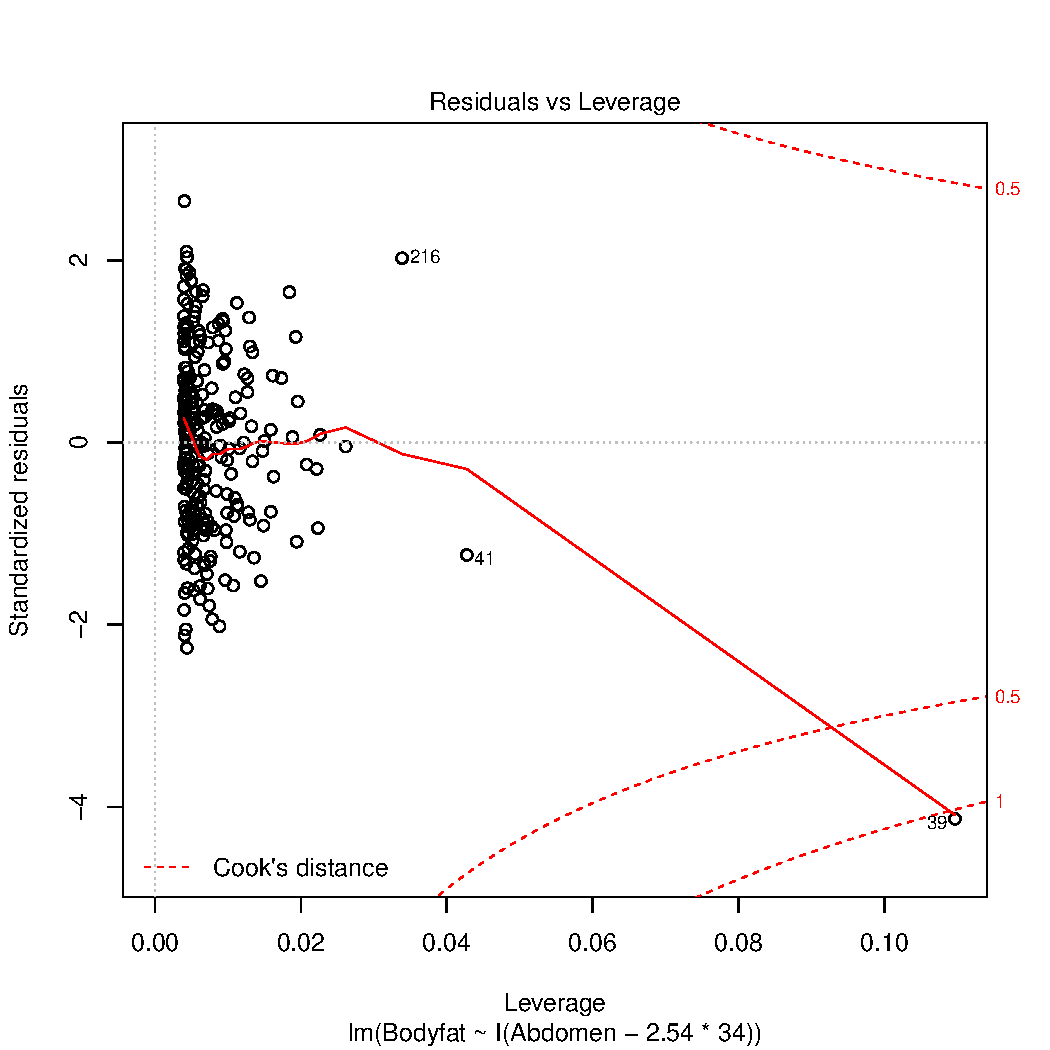
\includegraphics[height=3.5in]{CooksD}}

\end{frame}


  \begin{frame} \frametitle{Outliers in Regression}
    \begin{itemize}
    \item Hoeting, Madigan and Raftery (in various permutations)
      consider the problem of simultaneous variable selection and
      outlier identification. \pause
\item   This is implemented in the package {\tt BMA} in the function
  {\tt MC3.REG}.
This has the advantage that more than 2 points may be considered as
outliers at the same time. \pause
\item The function uses a Markov chain to identify both important
  variables and potential outliers, but is coded in Fortran so should
  run reasonably quickly. \pause
\item Can also use BAS or other variable selection programs \pause
  \end{itemize}
  \end{frame}




\begin{frame} \frametitle{Options for Handling Influential Cases}
\begin{itemize}
\item Are there scientific grounds for eliminating the case? \pause
\item Test if the case  has a different mean than population \pause
\item Report results with and without the case \pause
\item Model Averaging to Account for Model Uncertainty?  \pause

\item Full model $\Y = \X \b + \I_n\d + \epsilon$ \pause
\item $2^n$ submodels $\gamma_i = 0 \Leftrightarrow \delta_i = 0$
\item If $\gamma_i = 1$ then case $i$ has a different mean ``mean
  shift'' outliers.
\end{itemize}

\end{frame}


\begin{frame}
  \frametitle{Mean Shift $=$ Variance Inflation}
  \begin{itemize}
  \item Model  $\Y = \X \b + \I_n\d + \epsilon$

\item Prior \\
$\qquad \delta_i \mid \gamma_i \sim N(0, V \sigma^2 \gamma_i)$ \\
$\qquad \gamma_i \sim  \Ber(\pi)$
  \end{itemize}



Then $\epsilon_i$ given $\sigma^2$ is independent of $\delta_i$
and
$$\epsilon^*_i \equiv \epsilon_i + \delta_i \mid \sigma^2 \left\{
\begin{array}{llc}
  N(0, \sigma^2) & wp &(1 - \pi) \\
  N(0, \sigma^2(1 + V)) & wp & \pi
\end{array}
\right.
$$

Model  $\Y = \X \b + \epsilon^*$   ``variance inflation'' \\

$V+1 = K = 7$ in the paper by Hoeting et al. package {\tt BMA}
\end{frame}
\begin{frame}[fragile]
  \frametitle{Simultaneous Outlier and Variable Selection}
  \begin{small}
\begin{verbatim}
MC3.REG(all.y = bodyfat$Bodyfat, all.x = as.matrix(bodyfat$Abdomen),
        num.its = 10000, outliers = TRUE)

Model parameters: PI=0.02 K=7 nu=2.58 lambda=0.28 phi=2.85

  15  models were selected
 Best  5  models (cumulative posterior probability =  0.9939):

           prob    model 1  model 2  model 3  model 4  model 5
variables
  all.x    1         x        x        x        x        x
outliers
  39       0.94932   x        x        .        x        .
  204      0.04117   .        .        .        x        .
  207      0.10427   .        x        .        .        x

post prob         0.815    0.095    0.044    0.035    0.004
\end{verbatim}

  \end{small}

\end{frame}


\begin{frame} \frametitle{Change Error Assumptions}
\vspace{-.25in}
\begin{eqnarray*}
Y_i & \ind & t(\nu, \alpha + \beta x_i, 1/\phi)\\ \pause
L(\alpha, \beta,\phi) & \propto & \prod_{i = 1}^n \phi^{1/2} \left(1 +
\frac{\phi (y_i - \alpha - \beta x_i)^2}{\nu}\right)^{-\frac{(\nu +
  1)}{2}}
\end{eqnarray*} \pause
Use Prior $p(\alpha, \beta, \phi) \propto 1/\phi$ \pause

\bigskip
Posterior distribution
$$ p(\alpha, \beta, \phi \mid Y) \propto \phi^{n/2 - 1} \prod_{i = 1}^n  \left(1 +
\frac{\phi (y_i - \alpha - \beta x_i)^2}{\nu}\right)^{-\frac{(\nu +
  1)}{2}}$$ \pause

\end{frame}

\begin{frame}
  \frametitle{Bounded Influence - West 1984 (and references within)}
  Treat $\sigma^2$ as given,  then {\it influence} of individual observations on the posterior distribution of $\b$  in the model where $\E[\Y_i] = \x_i^T\b$ is investigated through the score function: \pause

$$
\frac{d} {d \b} \log p (\b \mid \Y) = \frac{d} {d \b} \log p(\b) +  \sum_{i = 1}^n \x_i g(y_i - \x^T_i \b)
$$ \pause
where
$$ g(\eps) = - \frac{d} {d \eps} \log p(\eps)
$$
is the influence function of the error distribution (unimodal, continuous, differentiable, symmetric)
\pause

\vspace{10pt}
An outlying observation $y_j$ is accommodated if the posterior distribution for $p(\b \mid \Y_{(i)})$ converges to $p(\b \mid \Y)$  for all $\b$ as $|\Y_i| \to \infty$.   Requires error models with influence functions that go to zero such as the Student $t$ (O'Hagan, 1979)
\end{frame}

\begin{frame} \frametitle{Choice of df}

  \begin{itemize}
  \item  Score function for $t$ with $\alpha$ degrees of freedom has turning points at $\pm \sqrt{\alpha}$ \pause

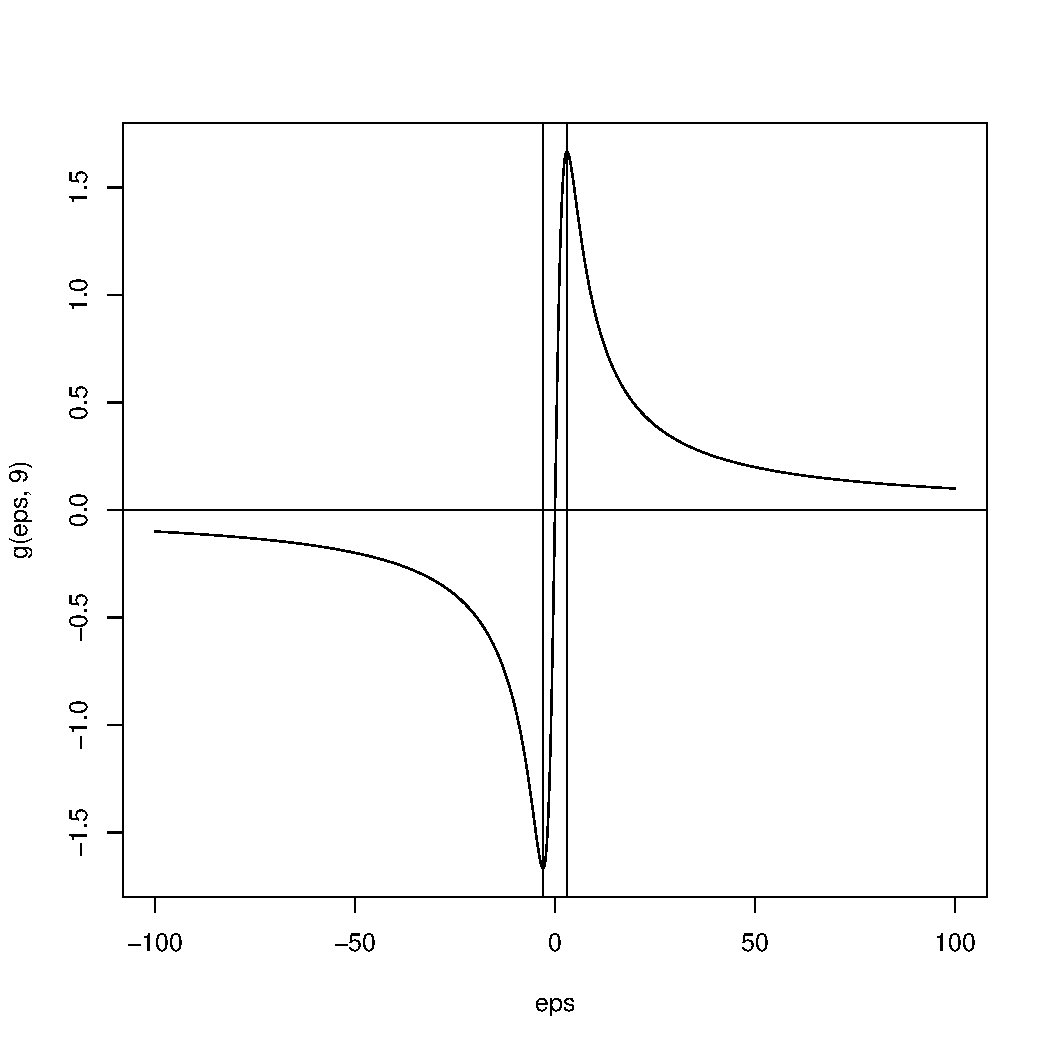
\includegraphics[height=2in]{influence}

\item $g'(\eps) $ is negative when $\eps^2 > \alpha$  (standardized errors) \pause
\item Contribution of observation to information matrix is negative and the observation is doubtful \pause
\item Suggest taking $\alpha = 8$ or $\alpha = 9$ to reject errors larger than $\sqrt{8}$ or $3$ sd. \pause

  \end{itemize}

Problem:   No closed form solution for posterior distribution
\end{frame}


\begin{frame} \frametitle{Scale-Mixtures of Normal Representation}
\begin{eqnarray*}
Z_i \simiid t(\nu, 0, \sigma^2)   \Leftrightarrow  &  &\pause\\
& & Z_i \mid \lambda_i \ind N(0, \sigma^2/\lambda_i) \pause \\
& & \lambda_i \simiid G(\nu/2, \nu/2) \pause
\end{eqnarray*}
Integrate out ``latent'' $\lambda$'s to obtain marginal distribution.

\end{frame}  \begin{frame} \frametitle{Latent Variable Model}
\begin{eqnarray*}
  Y_i \mid \alpha, \beta, \phi, \lambda & \ind & N(\alpha + \beta x_i,
  \frac{1}{\phi \lambda_i}) \pause\\
 \lambda_i & \simiid & G(\nu/2, \nu/2) \pause\\
 p(\alpha, \beta, \phi) & \propto & 1/\phi  \pause
\end{eqnarray*}

Joint Posterior Distribution: \pause
\begin{eqnarray*}
p((\alpha, \beta, \phi, \lambda_1, \ldots, \lambda_n \mid Y)
  \propto \,  & &
\phi^{n/2} \exp\left\{ - \frac{\phi}{2} \sum \lambda_i(y_i - \alpha
  - \beta x_i)^2 \right\} \times \pause \\
&  & \phi^{-1} \pause \\
&  &\prod_{i=1}^n \lambda_i^{\nu/2 - 1} \exp(- \lambda_i \nu/2)
\end{eqnarray*}
\end{frame}



\begin{frame}[fragile]
\frametitle{Model Specification via R2jags}
\begin{verbatim}
rr.model = function() {
  for (i in 1:n) {
    mu[i] <- alpha0 + alpha1*(X[i] - Xbar)
    lambda[i] ~ dgamma(9/2, 9/2)
    prec[i] <- phi*lambda[i]
    Y[i] ~ dnorm(mu[i], prec[i])
  }
  phi ~ dgamma(1.0E-6, 1.0E-6)
  alpha0 ~ dnorm(0, 1.0E-6)
  alpha1 ~ dnorm(0,1.0E-6)
}
\end{verbatim}
\end{frame}


\begin{frame}[fragile] \frametitle{Specifying which Parameters to Save}
The parameters to be monitored and returned to R are specified with
the variable {\tt parameters}

\begin{verbatim}
parameters = c("beta0", "beta1", "sigma",
               "mu34", "y34", "lambda[39]")
\end{verbatim}
\begin{itemize}
\item All of the above (except lambda) are calculated from the other
  parameters. (See R-code for definitions of these parameters.) \pause
\item {\tt mu34} and {\tt y34} are the mean functions and predictions for a man with a 34 in waist.
\item {\tt lambda[39]} saves only the 39th case of $\lambda$ \pause
\item  To save a whole vector (for example all lambdas, just give the
  vector name) \pause
\end{itemize}
\end{frame}



\begin{frame} \frametitle{Output}
\begin{table}[ht]
\begin{center}
\begin{tabular}{rrrrrr}
  \hline
 & mean & sd & 2.5\% & 50\% & 97.5\% \\
  \hline
beta0 & -41.70 & 2.75 & -46.91 & -41.67 & -36.40 \\
  beta1 & 0.66 & 0.03 & 0.60 & 0.66 & 0.71 \\
  sigma & 4.48 & 0.23 & 4.05 & 4.46 & 4.96 \\
  mu34 & 15.10 & 0.35 & 14.43 & 15.10 & 15.82 \\
  y34 & 14.94 & 5.15 & 4.37 & 15.21 & 24.65 \\
  lambda[39] & 0.33 & 0.16 & 0.11 & 0.30 & 0.72 \\
   \hline
\end{tabular}
\end{center}
95\% HPD interval for expected bodyfat $(14.5, 15.8)$ \\
95\% HPD interval for bodyfat $(5.1, 25.3)$

\end{table}
\end{frame}

\begin{frame} \frametitle{Comparison}
\begin{itemize}
\item  95\% Probability Interval for $\beta$ is $(0.60, 0.71)$ with
  $t_9$ errors \pause
\item 95\% Confidence Interval for $\beta$ is $(0.58, 0.69)$
(all data normal model)  \pause
\item 95\% Confidence Interval for $\beta$ is $(0.61, 0.73)$
( normal model without case 39) \pause
\end{itemize}
Results intermediate without having to remove any observations
\pause
\vspace{.2in}
Case 39 down weighted by $\lambda_{39}$

\end{frame}


\begin{frame} \frametitle{Full Conditional for $\lambda_j$}
\begin{eqnarray*}
p(\lambda_j \mid \text{rest}, Y) & \propto &
p(\alpha, \beta, \phi, \lambda_1, \ldots, \lambda_n \mid Y) \pause \\
 &
\propto & \phi^{n/2 - 1}  \prod_{i=1}^n \exp\left\{ - \frac{\phi}{2}  \lambda_i(y_i - \alpha
  - \beta x_i)^2 \right\} \times \\
&  &\quad \prod_{i=1}^n \lambda_i^{\frac{\nu+1}{2} - 1} \exp(- \lambda_i
\frac{\nu}{2})
\end{eqnarray*}\pause

Ignore all terms except those that involve $\lambda_j$ \pause

\bigskip
$$\lambda_j \mid \text{rest}, Y \sim G \left(\frac{\nu + 1}{2}, \frac{\phi(y_j - \alpha -
\beta x_j)^2 + \nu}{2} \right)$$
\end{frame}

 \begin{frame} \frametitle{Weights}
Under prior $E[\lambda_{i}] = 1$  \pause

Under posterior, large residuals are down-weighted (approximately
those bigger than $\sqrt{\nu}$)

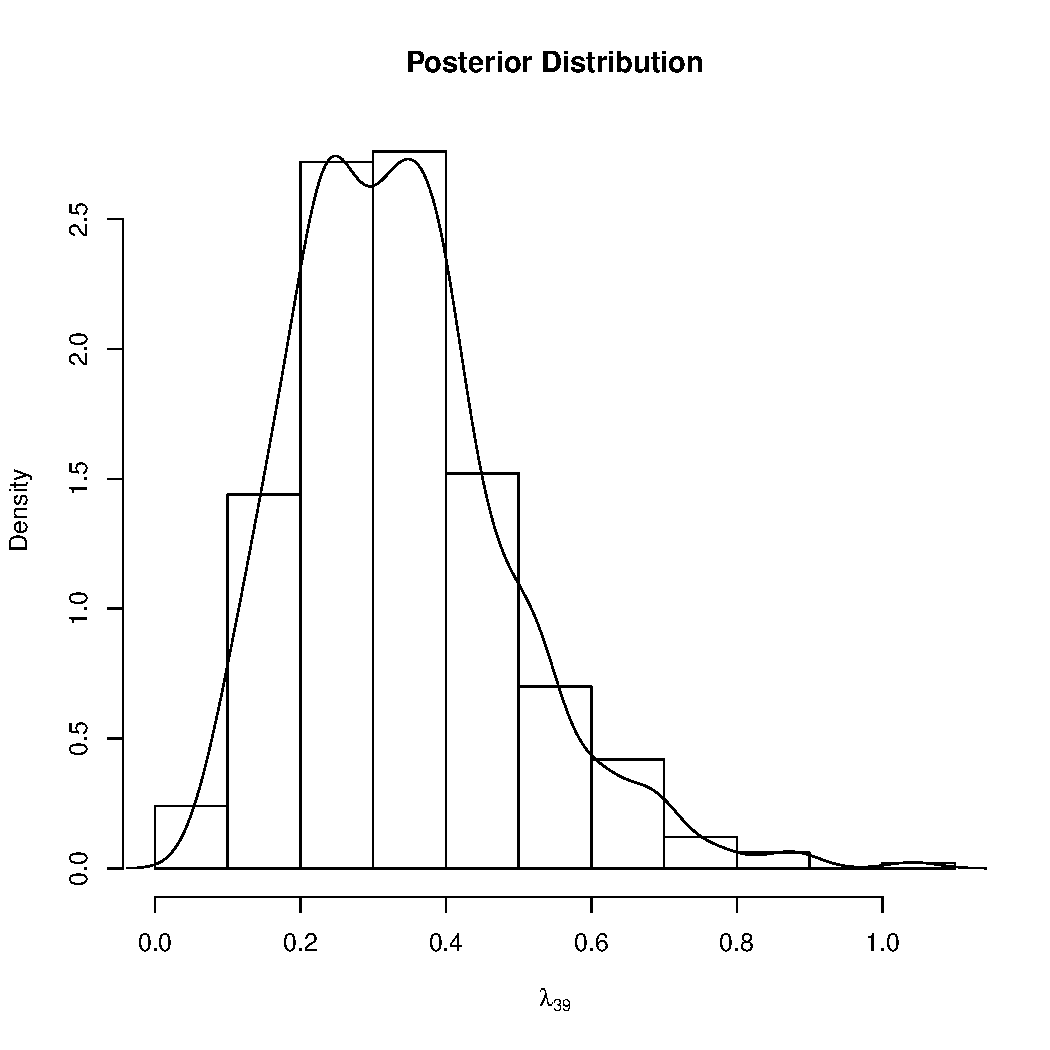
\includegraphics[height=2.5in]{lambda39}

\end{frame}
\begin{frame}
  \frametitle{Prior Distributions on Parameter}

As a general recommendation, the prior distribution should have
``heavier'' tails than the likelihood \pause
\begin{itemize}
\item with $t_9$ errors use a $t_\alpha$ with $\alpha < 9$ \pause
\item also represent via scale mixture of normals \pause
\item Horseshoe, Double Pareto, Cauchy all have heavier tails \pause
\end{itemize}
\end{frame}




\begin{frame} \frametitle{Sumary}
\begin{itemize}
  \item Classical diagnostics useful for EDA (checking data, potential outliers/influential points) or posterior predictive checks
  \item BMA/BVS and Bayesian robust regression avoid interactive decision making about outliers
  \item Robust Regression (Bayes) can still identify outliers through distribution on weights

  \item continuous versus mixture distribution on scale parameters

  \item Other mixtures (sub populations?) on scales and $\b$?

\end{itemize}

\end{frame}
\end{document}


